% This file was created with tikzplotlib v0.10.1.post5.
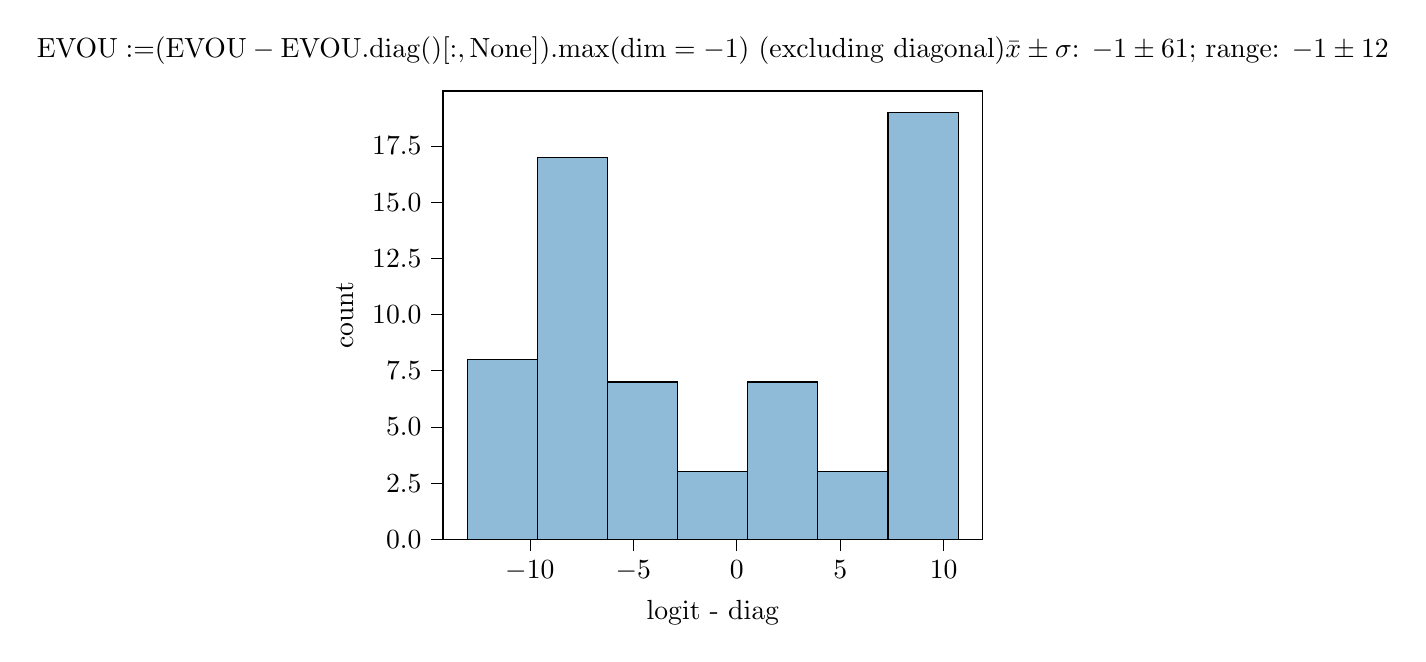
\begin{tikzpicture}

\definecolor{darkgray176}{RGB}{176,176,176}
\definecolor{steelblue31119180}{RGB}{31,119,180}

\begin{axis}[
tick align=outside,
tick pos=left,
title={\(\displaystyle \mathrm{EVOU} := \WE \WV \WO\WU \)\\
\(\displaystyle (\mathrm{EVOU} - \mathrm{EVOU}\mathrm{.diag}()[:,\mathrm{None}])\mathrm{.max}(\mathrm{dim}=-1)\) (excluding diagonal)\\
\(\displaystyle \bar{x}\pm\sigma\): \(\displaystyle -1 \pm 61\); range: \(\displaystyle -1 \pm 12\)},
x grid style={darkgray176},
xlabel={logit - diag},
xmin=-14.1964001655579, xmax=11.881151676178,
xtick style={color=black},
xtick={-15,-10,-5,0,5,10,15},
xticklabels={
  \(\displaystyle {\ensuremath{-}15}\),
  \(\displaystyle {\ensuremath{-}10}\),
  \(\displaystyle {\ensuremath{-}5}\),
  \(\displaystyle {0}\),
  \(\displaystyle {5}\),
  \(\displaystyle {10}\),
  \(\displaystyle {15}\)
},
y grid style={darkgray176},
ylabel={count},
ymin=0, ymax=19.95,
ytick style={color=black},
ytick={0,2.5,5,7.5,10,12.5,15,17.5,20},
yticklabels={
  \(\displaystyle {0.0}\),
  \(\displaystyle {2.5}\),
  \(\displaystyle {5.0}\),
  \(\displaystyle {7.5}\),
  \(\displaystyle {10.0}\),
  \(\displaystyle {12.5}\),
  \(\displaystyle {15.0}\),
  \(\displaystyle {17.5}\),
  \(\displaystyle {20.0}\)
}
]
\draw[draw=black,fill=steelblue31119180,fill opacity=0.5] (axis cs:-13.0110569000244,0) rectangle (axis cs:-9.62436185564314,8);
\draw[draw=black,fill=steelblue31119180,fill opacity=0.5] (axis cs:-9.62436185564314,0) rectangle (axis cs:-6.23766681126186,17);
\draw[draw=black,fill=steelblue31119180,fill opacity=0.5] (axis cs:-6.23766681126186,0) rectangle (axis cs:-2.85097176688058,7);
\draw[draw=black,fill=steelblue31119180,fill opacity=0.5] (axis cs:-2.85097176688058,0) rectangle (axis cs:0.535723277500697,3);
\draw[draw=black,fill=steelblue31119180,fill opacity=0.5] (axis cs:0.535723277500697,0) rectangle (axis cs:3.92241832188197,7);
\draw[draw=black,fill=steelblue31119180,fill opacity=0.5] (axis cs:3.92241832188197,0) rectangle (axis cs:7.30911336626325,3);
\draw[draw=black,fill=steelblue31119180,fill opacity=0.5] (axis cs:7.30911336626325,0) rectangle (axis cs:10.6958084106445,19);
\end{axis}

\end{tikzpicture}
